%-------------------------------------------------------------------
\chapter{\textbf{Fast Supercapacitor Charger for SCATMA}}
\label{ch:Charger_basics}
%-------------------------------------------------------------------

\section{Fast Charging Requirement in SCATMA}
As described in previous chapters, ``instant" water heating requires stored energy that can be delivered at a fast rate. The hybrid solution based on a SC/battery series-hybrid arrangement as described in Chapter~\ref{ch:prototype} has the major drawback that the size of the required energy storage is too big. Compared with SCs, batteries have a very short cycle life~(one million deep discharge cycles for SCs vs a maximum of 1000--2000 for batteries\cite{Schneuwly:00}). 

%-------------------------------------------------------------------
\subsection{Energy Balance}
Based on the average specifications of ``instant" water heating, 100--150~Wh of energy is required for the 30~s period of operation. A SC bank providing up to 50~Wh is feasible based on cost and size. Possible options for the rest of the energy requirement are

\begin{enumerate}
	\item to draw more than 10 A from the mains supply for a short period of time without overloading the wiring or tripping the protective circuit breaker.  
	\item to draw the nominal 2.3~kW from the mains supply. This can be used for the time after the mains supply has had its 10 A supply exceeded by the previous option.
	\item to store energy by a cheaper alternative than SCs (such as a battery). Such a store can have a lower power density but a higher energy density than SCs.
\end{enumerate}



Given the availability of these options the problem lies in how this energy can be delivered to the load with galvanic isolation and at the required 15--18~kW average power level. For both of these conditions to be satisfied, a SC bank circulation technique first proposed for surge resistant uninterrupted power supply~(SRUPS)\cite{SRUPS:11, Madawala:2007} is used.

\subsection {SRUPS}    

 The first scenario is for charging a capacitor fully discharged from a voltage source at the capacitor rated voltage. This method loses the same amount of energy as stored in the capacitor in the lumped resistor irrespective of the value of the total resistance of the charging path. The second scenario is charging a partially discharged capacitor from a voltage source at the capacitor rated voltage. The losses are dependant on the start factor $n$ and they vary as seen in, the best charging efficiency is achieved when $E_C - E_R$ maximises. That is when the first derivative of $E_C - E_R$ with respect to $n$ becomes zero:


\begin{figure}[h]
	\centering
	\resizebox{16cm}{!}{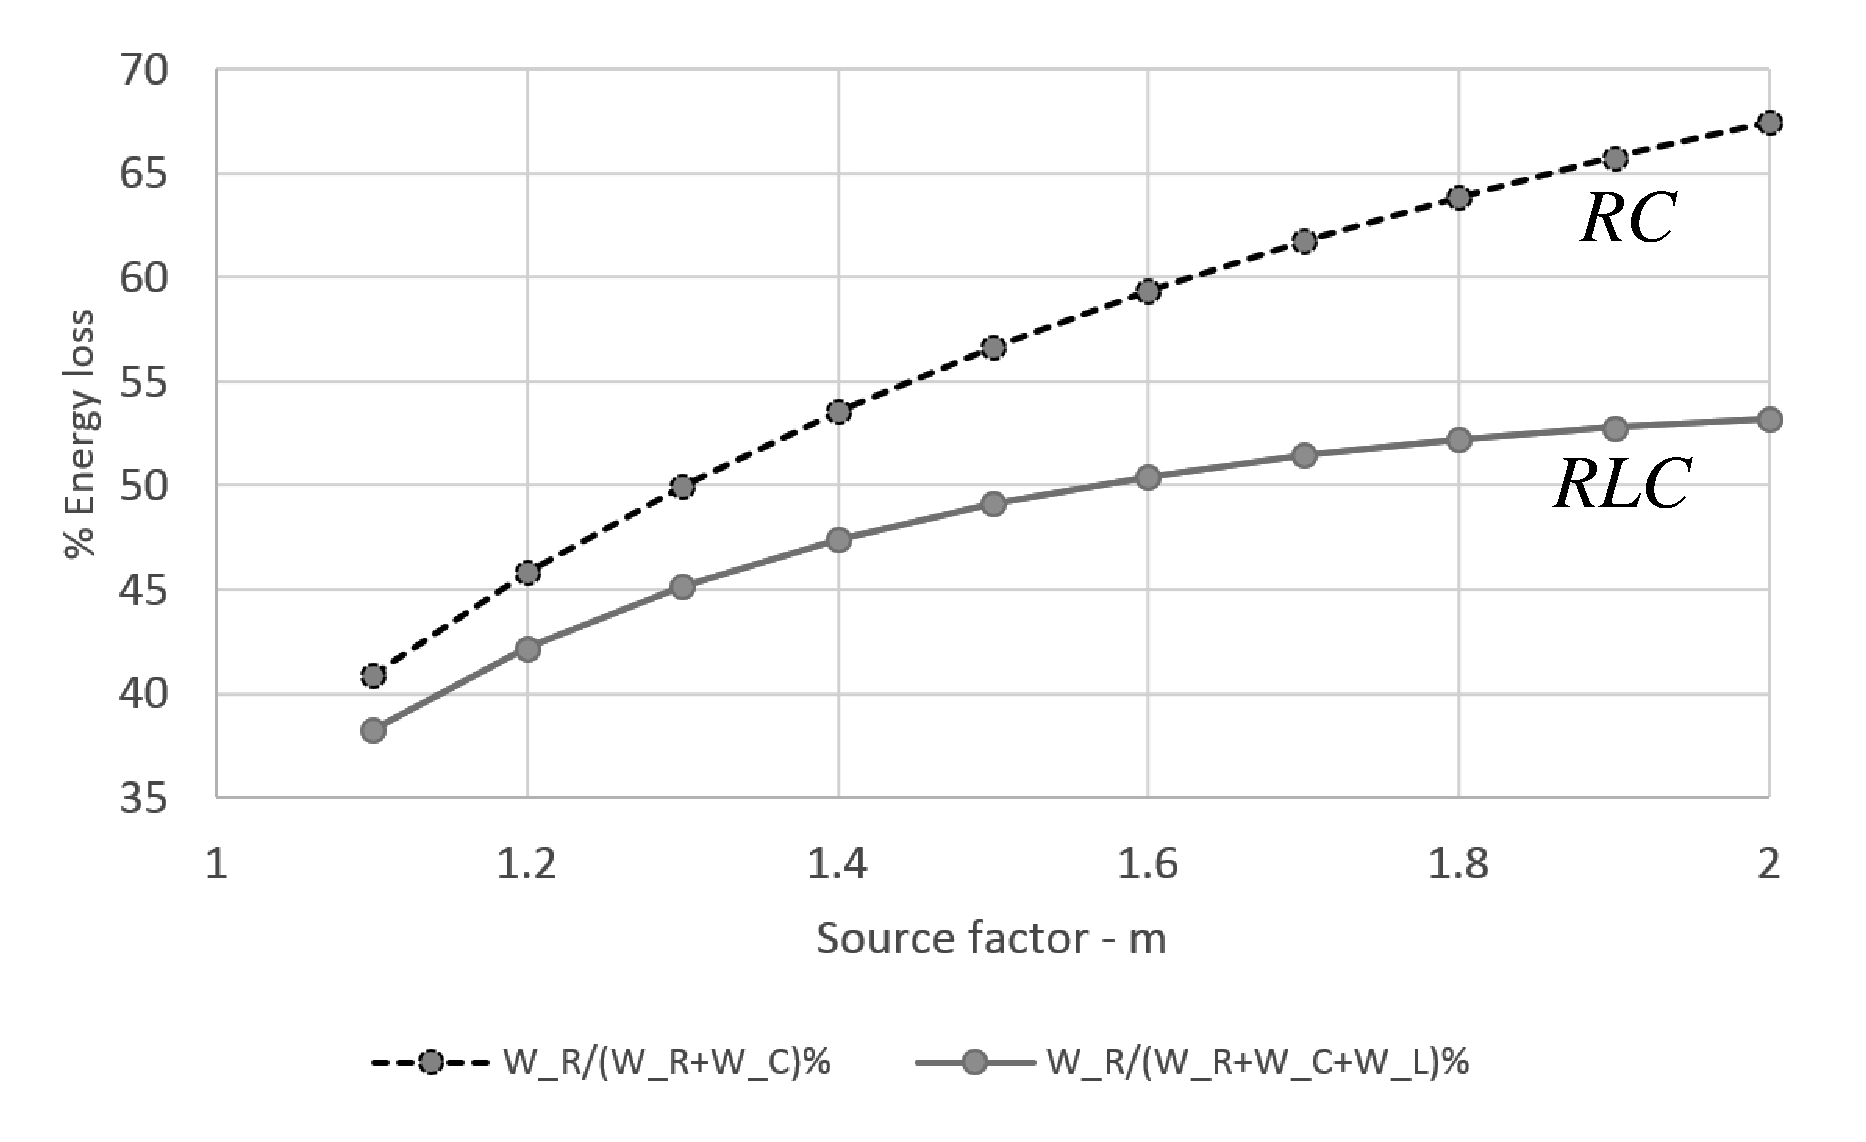
\includegraphics[draft=false]{_figs/RC_RLC_advantage_sim.pdf}}
	%\includegraphics[draft=false]{_figs/Ragone_plot}
	\caption[Efficiency improvement of a $RLC$ system]
	{%
		\label{fg:RC_RLC_advantage_sim}
		\centering
		Efficiency improvement of a $RLC$ system over a $RC$ system for $m$-times charging ($C = 310~$F$, L = 2$ mH, $R = 50~$m$\Omega, V_C = 2.7 $V, $n = 0.3$)}
\end{figure}





